\documentclass[11pt]{article}

\usepackage{times}
\usepackage{epsf}
\usepackage{epsfig}
\usepackage{amsmath, alltt, amssymb, xspace}
\usepackage{wrapfig}
\usepackage{fancyhdr}
\usepackage{url}
\usepackage{verbatim}
\usepackage{fancyvrb}
\usepackage{float}

\usepackage{subfigure}
\usepackage{cite}
\usepackage{hyperref}
\hypersetup{%
    pdfborder = {0 0 0}
}
\topmargin      -0.50in  % distance to headers
\oddsidemargin  0.0in
\evensidemargin 0.0in
\textwidth      6.5in
\textheight     8.9in 


%\centerfigcaptionstrue

%\def\baselinestretch{0.95}


\newcommand\discuss[1]{\{\textbf{Discuss:} \textit{#1}\}}
%\newcommand\todo[1]{\vspace{0.1in}\{\textbf{Todo:} \textit{#1}\}\vspace{0.1in}}
\newtheorem{problem}{Problem}[section]
%\newtheorem{theorem}{Theorem}
%\newtheorem{fact}{Fact}
\newtheorem{define}{Definition}[section]
%\newtheorem{analysis}{Analysis}
\newcommand\vspacenoindent{\vspace{0.1in} \noindent}

%\newenvironment{proof}{\noindent {\bf Proof}.}{\hspace*{\fill}~\mbox{\rule[0pt]{1.3ex}{1.3ex}}}
%\newcommand\todo[1]{\vspace{0.1in}\{\textbf{Todo:} \textit{#1}\}\vspace{0.1in}}

%\newcommand\reducespace{\vspace{-0.1in}}
% reduce the space between lines
%\def\baselinestretch{0.95}

\newcommand{\fixmefn}[1]{ \footnote{\sf\ \ \fbox{FIXME} #1} }
\newcommand{\todo}[1]{
\vspace{0.1in}
\fbox{\parbox{6in}{TODO: #1}}
\vspace{0.1in}
}

\newcommand{\mybox}[1]{
\vspace{0.2in}
\noindent
\fbox{\parbox{6.5in}{#1}}
\vspace{0.1in}
}


\newcounter{question}
\setcounter{question}{1}

\newcommand{\myquestion} {{\vspace{0.1in} \noindent \bf Question \arabic{question}:} \addtocounter{question}{1} \,}

\newcommand{\myproblem} {{\noindent \bf Problem \arabic{question}:} \addtocounter{question}{1} \,}



\newcommand{\copyrightnotice}[1]{
\vspace{0.1in}
\fbox{\parbox{6in}{
      This lab was developed for the Labtainer framework by the Naval Postgraduate 
      School, Center for Cybersecurity and Cyber Operations.
      This work is in the public domain, and cannot be copyrighted.}}
\vspace{0.1in}
}


\newcommand{\idea}[1]{
\vspace{0.1in}
{\sf IDEA:\ \ \fbox{\parbox{5in}{#1}}}
\vspace{0.1in}
}

\newcommand{\questionblock}[1]{
\vspace{0.1in}
\fbox{\parbox{6in}{#1}}
\vspace{0.1in}
}


\newcommand{\argmax}[1]{
\begin{minipage}[t]{1.25cm}\parskip-1ex\begin{center}
argmax
#1
\end{center}\end{minipage}
\;
}

\newcommand{\bm}{\boldmath}
\newcommand  {\bx}    {\mbox{\boldmath $x$}}
\newcommand  {\by}    {\mbox{\boldmath $y$}}
\newcommand  {\br}    {\mbox{\boldmath $r$}}


\newcommand{\tstamp}{\today}   
%\rfoot[\fancyplain{\tstamp} {\tstamp}]  {\fancyplain{}{}}

\pagestyle{fancy}
\lhead{\bfseries Labtainers}
\chead{}
\rhead{\small \thepage}
\lfoot{}
\cfoot{}
\rfoot{}




\begin{document}

\begin{center}
{\LARGE DMZ Example}
\vspace{0.1in}\\
\end{center}

\copyrightnotice

\section{Overview}
This lab illustrates a simple DMZ.
It is intended as an example network topology definition for
Labtainer exercises.

\section{Lab Environment}
This lab runs in the Labtainer framework,
available at http://my.nps.edu/web/c3o/labtainers.
That site includes links to a pre-built virtual machine
that has Labtainers installed, however Labtainers can
be run on any Linux host that supports Docker containers.

From your labtainer-student directory start the lab using:
\begin{verbatim}
    labtainer dmz-example
\end{verbatim}
\noindent A link to this lab manual will be displayed.  

\section{Network Configuration}
This lab includes several networked computers as shown in Figure~\ref{fig:topology}.
Note however that your instance of the lab will have different IP addresses
for some of the components.
When the lab starts, you will get several virtual terminals, one connected to each
component.

The DMZ is created using an inner gateway and an outer gateway.  The former uses NAT to
hide internal network addresses.

The outer gateway and the remote gateway each reach the Internet via an ISP with 
address 198.18.0.1.  The local site has a network address of 198.18.1.0/24.  The remote
site has a network address of 203.0.113.0/24.

\begin{figure}[htb]
\begin{center}
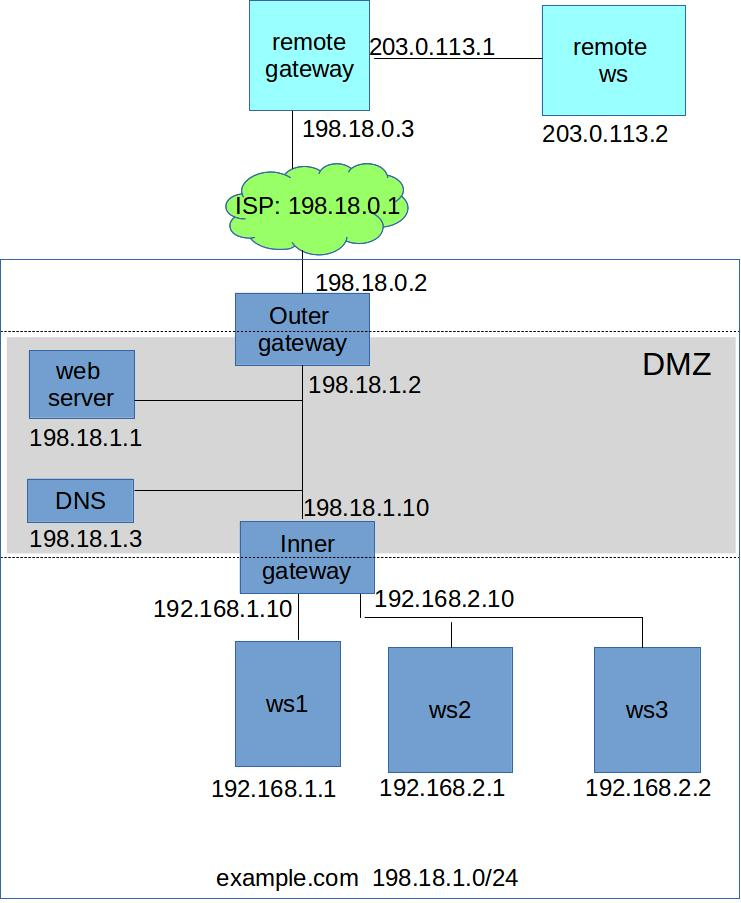
\includegraphics [width=0.8\textwidth,natwidth=621,natheight=403]{dmz-example.jpg}
\end{center}
\caption{Network topology for dmz-example lab}
\label{fig:topology}
\end{figure}

\section{Lab Tasks}
Use nmap on various components within the lab to determine which services are visible from
different locations within the network topology.  Review the iptables configurations as
defined in the /etc/rc.local scripts on the inner and outer gateways.

\section{Submission}
After finishing the lab, go to the terminal on your Linux system that was used to start the lab and type:
\begin{verbatim}
    stoplab dmz-example
\end{verbatim}
When you stop the lab, the system will display a path to the zipped lab results on your Linux system.  Provide that file to 
your instructor, e.g., via the Sakai site.

\end{document}
